
\subsection{Vergleich der Wörterbücher auf Wochenebene}

Da mehrere Wörterbücher zur Verfügung stehen, ist es erforderlich mehr Informationen durch weiteres Testen über diese Wörterbücher zu gewinnen. Im Kapitel \ref{Woerterbuch} wurden die Tweets auf der Tweetebene berechnet. Diese Berechnungen werden jetzt auf eine Wochenebene angehoben. Für die Wörterbücher \textit{bing} und \textit{nrc} werden die positven und negativen Wörter pro Woche gezählt und miteinander verrechnet um einen Sentimentindex zu bilden. Die Wörterbücher \textit{nrc} und \textit{vader} besitzen bereits einen Score.
\begin{figure}[H]
	\centering
	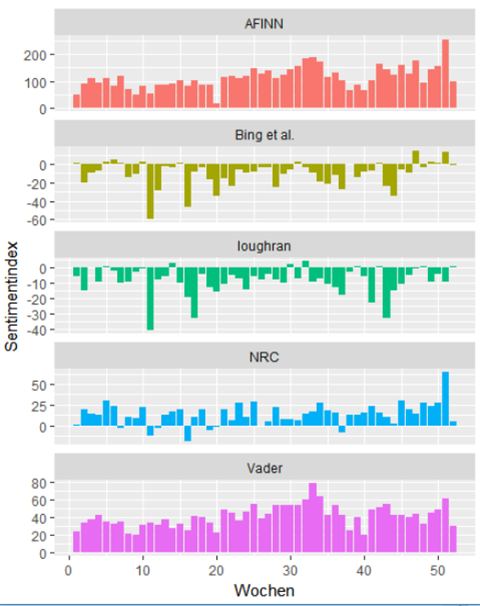
\includegraphics[width=1\textwidth]{Pictures/Woertbuch.png}
	\caption{Vergleich von Sentimentindizes der Wörterbücher \textit{Bing}, \textit{NRC}, \textit{Vader} und \textit{Afinn}, \textit{Loughran}}
	\label{senti}
\end{figure}
Die Abbildung \ref{senti} stellt die gegebenen Wörterbücher gegenüber und diese zeigen ähnliche Schwankungen zu entsprechenden Zeitpunkten. Das \textit{afinn}$\-$ und \textit{vader} Wörterbuch geben die größten absoluten Werte mit hohen positiven Werten an. Das Wörterbuch \textit{bing} und \textit{loughran} berechnen die niedrigsten Absolutwerte. Die \textit{nrc}- und \textit{vader}-Ergebnisse sind im Vergleich zu den anderen in der Höhe verschoben, wodurch der Text positivere Werte verzeichnet, aber ähnliche relative Veränderungen im Text erkannt werden. Wir finden geringfügige Unterschiede zwischen den Wörterbücher. Das \textit{nrc}-Sentiment weist hohe Absolutwerte auf, wohingegen das \textit{afinn}-Sentiment mehr Varianz aufweist. \textit{vader} hat ein ähnliches Verhalten, wie das \textit{nrc}-Sentiment. Die \textit{bing} und \textit{loughran} Sentimentindizes scheinen Wochen, die Nahe bei einander liegen, ähnlichen zu bewerten. Alle fünf Wörterbücher weisen unabhängig von ihren Sentimentindizes eine ähnliche Tendenz auf.

An dieser Stelle haben wir uns gefragt, warum das Ergebnis für das \textit{nrc} im Vergleich zum \textit{bing} eine positivere Stimmung aufweist? Diesbezüglich wird geprüft, wie viele positive und negative Wörter in diesen Wörterbüchern enthalten sind. Das Wörterbuch \textit{nrc} besitzt $3324$ negative und $2312$ positive Wörter. Im Gegensatz dazu beträgt das Wörterbuch \textit{bing} $4782$ negative und $2006$ positive Wörter, damit besitzt die Wörterliste \textit{bing} eine größere Anzahl von positiven Wörter. Diese unausgeglichenen der Klassen in den Wörterbücher können zu Problemen führen. 

\subsection{Übereinstimmungen von Sentimentindizes mit Aktienindizes}\label{ueberein}
In diesem Abschnitt wird ein Resume gezogen, inwieweit sich der Sentimentindex der Bankentweets aus $2012$ in der USA und der EU mit der wirtschaftlichen Situation in $2012$ übereinstimmt. 

% Für den Vergleich der wirtschaftlichen Situation in der EU, wird der \textit{EURO-STOXX} $50$ herangezogen. Der \textit{EURO-STOXX} $50$ ist ein Aktienindex, der sich aus den $50$ größten, börsennotierten Unternehmen des Euro-Währungsgebiets zusammensetzt. Der Dow Jones wird für die US-Banken-Tweets genommen. 

Um ein Bild der Stimmung in den Tweets zu erhalten, wird die Anzahl der positiven und negativen Wörter pro Monat gezählt und die Differenz berechnet. Für das Sentiment wurde das Wörterbuch \textit{bing} verwendet.
\begin{figure}[H]
	\begin{minipage}[b]{.4\linewidth} % [b] => Ausrichtung an \caption
	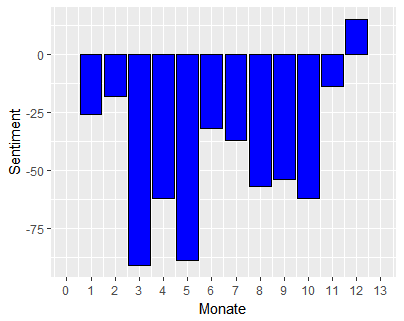
\includegraphics[width=1\textwidth]{Pictures/Monatusa.png}
	\caption{Sentimentindex USA-Banken Differenz  zwischen positven und negativen Wörtern pro Monat}\label{usadiff}
	
\end{minipage}
	\hspace{.2\linewidth}
\begin{minipage}[b]{.4\linewidth} % [b] => Ausrichtung an \caption
	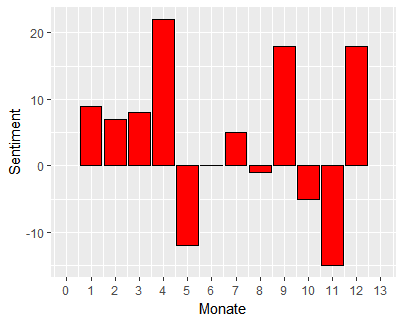
\includegraphics[width=1\textwidth]{Pictures/Monateu.png}
	\caption{Sentimentindex EU-Banken Differenz  zwischen positven und negativen Wörtern pro Monat}\label{eudiff}
\end{minipage}
\end{figure}
In Abbildung \ref{usadiff} ist die Differenz der Sentiments auf Monatsebene zu sehen. Dabei fällt auf, dass den Monaten von Januar bis November durchgehend negativ ausfallen. Die Sentiments des Balkendiagrammes \ref{eudiff} der EU-Banken sind sehr wechselhaft. Die Monate Mai, Juni, August, Oktober und November enthalten mehr negative als positive Wörter. Es werden die Höhen und Tiefen mit dem Aktienkurs des \textit{Dow Jones} und \textit{Euro Stoxx} $50$ aus $2012$ auf Gemeinsamkeiten untersucht.
 \begin{figure}[H]
 \begin{minipage}[b]{.4\linewidth} % [b] => Ausrichtung an \caption
 	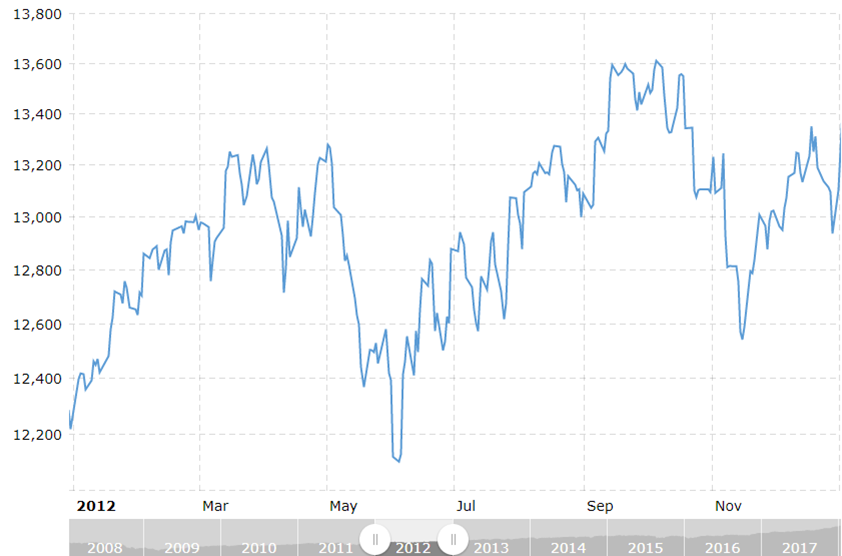
\includegraphics[width=1\textwidth]{Pictures/DowJones2012.png}
 	\caption{Dow Jones Aktienkurs 30 Industrial $2012$ \cite{Dow}}\label{dowjones}
 \end{minipage}
 \hspace{.2\linewidth}% Abstand zwischen Bilder
 \begin{minipage}[b]{.4\linewidth} % [b] => Ausrichtung an \caption
 	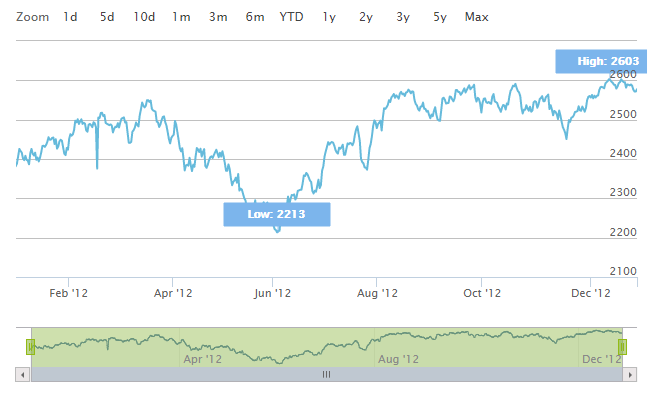
\includegraphics[width=1\textwidth]{Pictures/EuroxStoxx.png}
 	\caption{Euro Stoxx $50$ Aktienkurs $2012$ \cite{eurostoxx}} \label{eustoxx}
 \end{minipage}

\end{figure}
Der \textbf{Euro Stoxx} Chart zeigt in den Monaten Mai und Juni einen Kurssturz an und im August eine Erholung. Diese Informationen stimmen mit den Sentiments der Tweets überein. In der Phase des Aktiensturzes, die sich im Mai abzeichnet, existiert ein starker Anstieg an negativen Tweets. Im Juni ist der Tiefstand erreicht und der Aktienkurs steigt wieder an. Die Anzahl der negativen Wörtern ist leicht zurückgegangen und die Anzahl der positiven Wörtern angestiegen. Im August ist ein Aktieneinbruch zu erkennen. Dieser Effekt spiegelt sich auch in unseren Sentiments wieder. Es existieren gering mehr negative als positive Wörter im August. Dies lässt erahnen, dass dieser kurze Aktieneinsturz im August eine erhebliche Reaktion an negativen Tweets auslöste. In der Grafik \ref{eustoxx} zeichnet sich weiterhin im September eine Trendphase ungefähr bis Oktober ab. Dieser Trend scheint ebenfalls in den Tweets sichtbar zu werden, da mehr positive als negative Wörter im September vorhanden sind. 

Auch der Aktienkurs des Dow Jones (\ref{dowjones}) und der Sentimentindex der Tweets der \textbf{US-Banken} (\ref{usadiff}) aus $2012$ weisen Parallelen auf. Im März und im April steigt die Anzahl von negativen Wörtern stark an, wie in der Grafik \ref{usadiff} zu erkennen ist und nimmt nach Mai verstärkt wieder ab. Dieser Effekt stimmt mit dem Verhalten des Aktienkurs des Dow Jones überein. Im März und Mai existiert ein Einbruch und anschließend einen Trend. Die Stimmung in der Finanzwelt kann grob durch das Zählen von positiv und negativen Wörtern pro Monat erfasst werden. Im nächsten Abschnitt wird mittels verschiedener Sentimentindizes von mehreren Wochen eine multiple Regression auf wöchentliche Renditen durchgeführt.

\newpage

\section{Modell}\label{Modell}
Dieses Kapitel setzt statistische Grundlagen voraus, die im Bachelor der angewandten Mathematik in \textit{Statistik 1} und \textit{Statistik 2} behandelt wurden. Dieser Abschnitt bezieht seine Informationen aus der Literatur \cite{becker}. \\
\\
Einen gewissen Zusammenhang wurde zwischen einem einfachen Sentimentindex und der Rendite des Aktienindex Dow Jones im Kapitel \ref{ueberein} aufgezeigt. Der Sentimentindex zählt die positiven und negativen Sentiments der Tweets und nimmt als Score die Differenz. Im Rahmen der empirischen Untersuchung wird die klassische multiple Regression verwendet. Ziel der multiplen Regression auf wöchentliche Renditen von Aktienkursen ist es, die Kursentwicklung einer Aktie durch die Entwicklung eines zugehörigen Sentimentindexes zu erklären und vorherzusagen. Mittels den historischen Kursen \ref{sub:dow_jones_data} wird versucht ein Zusammenhang zwischen der Rendite (wöchentliche prozentuale Veränderung des Aktienindex) eines einzelnen Wertpapiers und einem Sentimentindex zu ermitteln. Durch dem gewonnen Zusammenhang können die zukünfitgen Renditen des Wertpapiers geschätzt werden.

Die künftigen Renditen der Aktienkurse werden ausschließlich durch den linearen Zusammenhang zu den Sentimentindizes der letzten Wochen geschätzt. Mit Hilfe einer multiplen linearen Einfachregression wird eine Schätzung für zukünftige Renditen des Aktienkurses erstellt, da ein linearer Zusammenhang zwischen der Rendite des einzelnen Wertpapiers und der Sentimentindizes vorausgesetzt wird. Es ergibt sich folgende lineare Regressionsgleichung:
\begin{equation}
r_{t}=\alpha_{t}+ \sum_{k=0}^{K} \beta_{t-k} S_{t-k}+\varepsilon_{t}
\end{equation}
mit:
\begin{itemize}
	\item  $r_{t}$ sind die wöchentlichen Renditen bzw. prozentuale Veränderung des Aktienkurses, für die $t$ Woche.
	\item $S_{t-k}$ ist der Sentimentindex der letzten $k$ Wochen und $\beta_{t-k}$ ist der dazugehörige Betakoeffizent für die $t$ Woche.
	\item $\alpha_{t}$ ist das Absolutglied der Woche $t$.
	\item $\varepsilon_{t}$ repräsentiert den Fehlerterm.
\end{itemize}
Im Folgendem wird versucht mit verschiedenen Sentimentindizes auf den \textit{Dow Jones Industrial} $30$ Renditen vorherzusagen. Da es den Rahmen dieser Ausarbeitung sprengen würde alle Ergebnisse der verschiedenen Regressionsansätzen aufzuzeigen und zu interpretieren, beschränkt sich dieser Abschnitt auf eine Regressionen. Wir verwenden als Sentimentindex den Mittelwert des \textit{afinn}-Scores der wöchentlichen US-Banken-Tweets. Der Sentimentindex wird mit dem Wörterbuch \textit{afinn} erstellt. Darauf wenden wir die multiple Regression an. Das Dataframe mit den Indizes muss mit dem Dataframe der Renditen des \textit{Dow Jones Inustrial} $30$  über das Feld \textit{week} gejoint werden. Für die Modellierung der Regressionsgleichung ist es erforderlich, sich zu überlegen, inwieweit der linearen Zusammenhang der Rendite zu den Sentimentindizes der letzten Wochen sinnvoll ist.\\
% Kannst du den Satz nochmal umschreiben "Für die Modellierung... TODO"
\\
\textbf{Wie viele Wochen ($K$) der Vergangenheit vom heutigen Zeitpunkt müssen in die Analyse einfließen, damit keine wichtigen Informationen verloren gehen?} 
\\
\\
Dies kann empirisch ermittelt werden. In unserem Fall gehen wir von der Hypothese aus, dass wir ein Zeitfenster von drei bis vier Wochen verwenden. Im nächsten Schritt wird eine Regression mit den Sentimentindizes der letzten drei Wochen durchgeführt. Hierzu muss das Dataframe dementsprechend transformiert werden. In Abbildung \ref{Afinn_summary} sind die Ergebnisse der Regression zusehen. Auf den ersten Blick fällt auf, dass nach dem $t$-Test alle $H_{0}$ Hypothesen für die Regressionskoeffizienten nicht verworfen werden können, da alle $\alpha>0.05$ sind, wie in der Tabelle \textit{Coefficients} in der Spalte $Pr(>|t|)$ zusehen ist. Die Sentimentinidizes der letzten drei Wochen besitzen keinen Einfluss auf die Renditen des \textit{Dow Jones Industrial} $30$. Das $R^2$ beträgt $3,84$ \% und weist den Prozentsatz aus, die die Regression an den Renditen erklären kann. Diese Ergebnisse sind nicht ungewöhnlich, da wir uns nicht in der normalen multiplen Regression bewegen, sondern im Bereich der Zeitreihenanalyse.
 \begin{figure}[H]
	\centering
	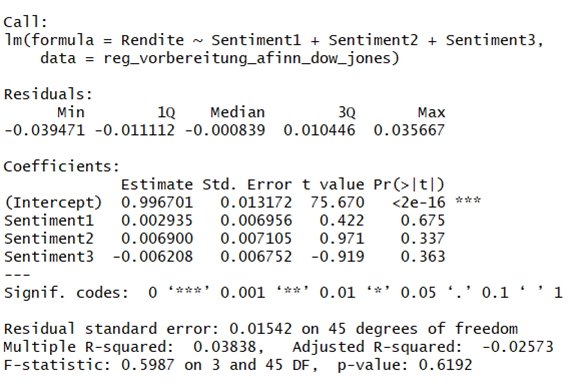
\includegraphics[width=1\textwidth]{Pictures/afinn_summary.png}
	\caption{Zusammenfassung der Regression mittels des Sentimentindex mit dem Wörterbuch \textit{Afinn} }
	\label{Afinn_summary}
\end{figure} 
\begin{figure}[H]
	\centering
	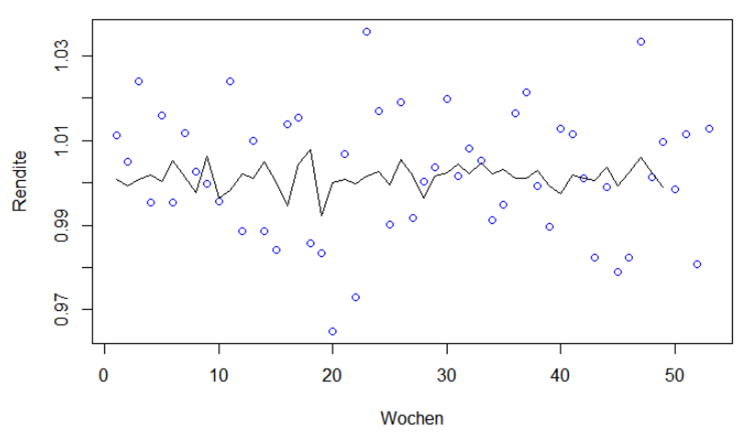
\includegraphics[width=1\textwidth]{Pictures/Afinn_plot.png}
	\caption{Regressions Plot des Sentimentindexes mit dem Wörterbuch \textit{Afinn} }
	\label{Afinn_plot_regression}
\end{figure} 
Weiterhin wurden verschiedene Ansätze der Regressionen durchgeführt. Einige von ihnen enthalten einen nicht linearen Ansatz, diese werden als Code im Anhang mitgeführt.  

